\chapter{Statistics and Experiments}

% =============================================================================
\section{Statistics}

\subsection{\texttt{STAT\_001} - Group Courses by Credits}

This experiment plots the number of courses for each possible number of credits
in a bars chart. The results of this was listed in
table~\ref{tab:courses_credits}.

\subsection{\texttt{STAT\_002} - List Domain of Courses Fields}

Gets domain of the fields of courses. Relevant results are listed in some
tables in section~\ref{sec:data_courses}.

% =============================================================================
\section{Experiments}

\subsection{\texttt{EXP\_001} - Plotting Activity of Students over the
Semester}

To look for patterns in the usage of Moodle we look into plotting the activity
of students over the courses over a semester. The six courses with the greatest
number of activities are chosen and for each of them two plots are made.

One plot displays the overall number of~\gls{crud} activities over the semester
and the number of \textbf{C}reate activities, \textbf{R}ead activities, etc.
Figure~\ref{fig:exp_001_all} show these plots for two courses. As it can be
seen, the number of Read activities is far greater then the others, which is to
be expected since to do any other activity, at least a Read activity has to
take place. For example, a student needs to open the Moodle page, and therefore
do a Read, to deliver a project, and therefore do a Create.

It is hypothesis that the number is also greater because students will usually
just read new messages in the Moodle, or consult new materials, without doing
any other activity.

The second plot made to each course is similar, but only the Create, Update,
and Delete activities are plotted. Figure~\ref{fig:exp_001_cud} show two
examples these plots. Notice that the number of creates is not always greater
then the number of updates, and vice-versa. But the number of deletes is always
below creates and updates. This concludes that the delete activity is simply
not that common.

\begin{figure}[h!]
    \centering

    \begin{subfigure}{.5\textwidth}
        \centering
        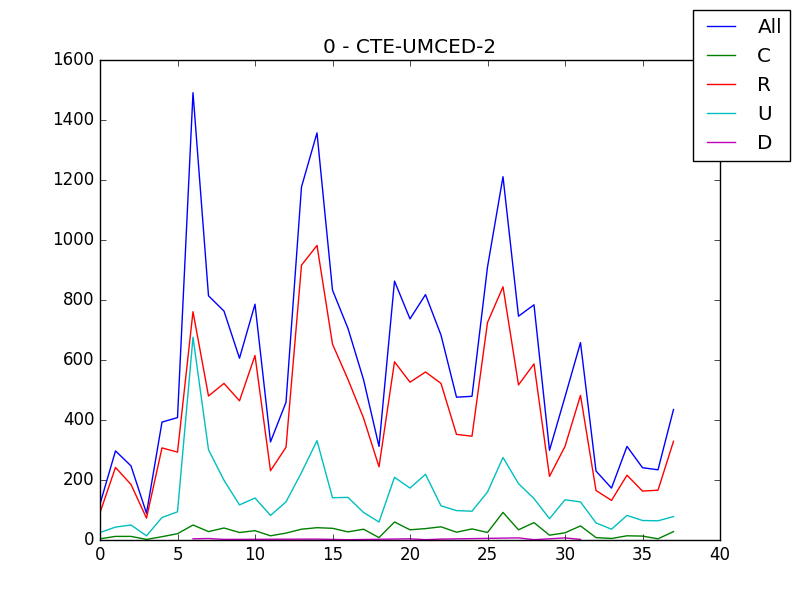
\includegraphics[width=\linewidth]{../src/exp_001_results/fig_0_CTE-UMCED-2_all}
        \label{subfig:exp_001_0_all}
    \end{subfigure}%
    \begin{subfigure}{.5\textwidth}
        \centering
        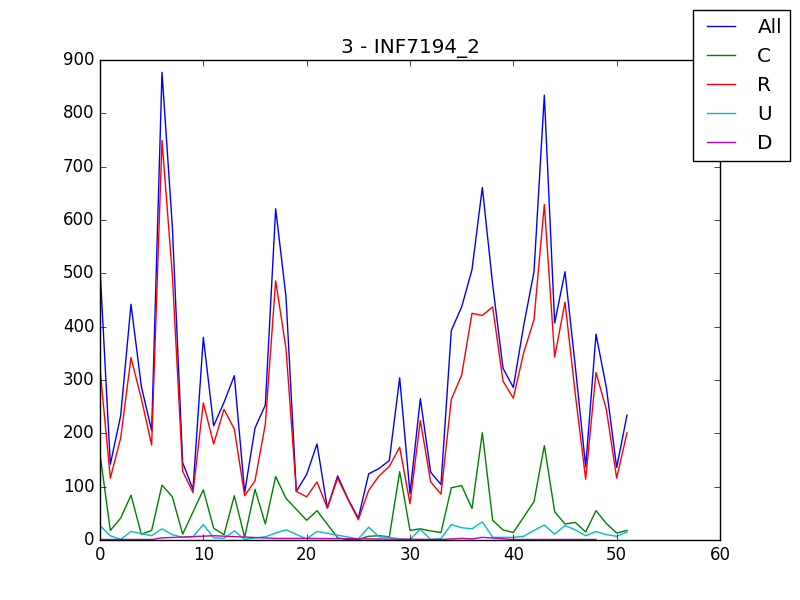
\includegraphics[width=\linewidth]{../src/exp_001_results/fig_3_INF7194_2_all}
        \label{subfig:exp_001_3_all}
    \end{subfigure}

    \caption
        [Exp 001 plots for all activities]
        {Exp 001 plots for all activities.}

    \label{fig:exp_001_all}
\end{figure}

\begin{figure}[h!]
    \centering

    \begin{subfigure}{.5\textwidth}
        \centering
        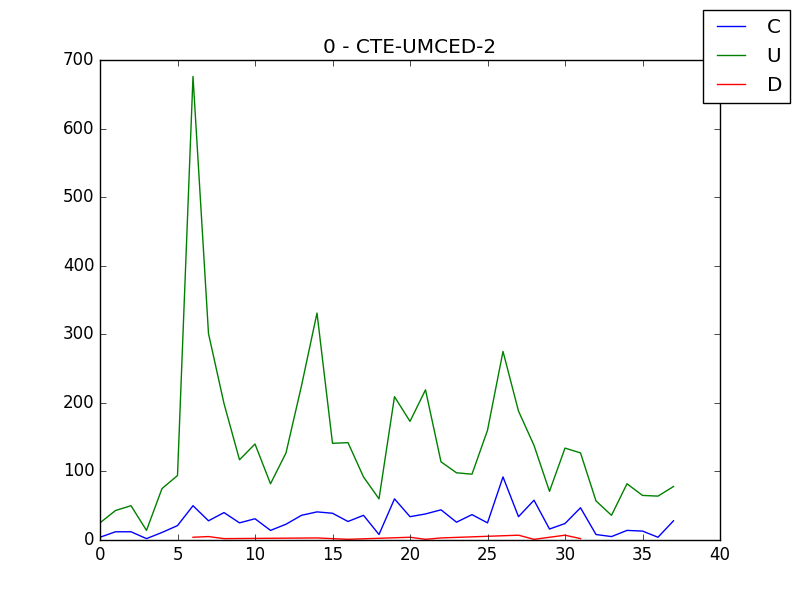
\includegraphics[width=\linewidth]{../src/exp_001_results/fig_0_CTE-UMCED-2_cud}
        \label{subfig:exp_001_0_cud}
    \end{subfigure}%
    \begin{subfigure}{.5\textwidth}
        \centering
        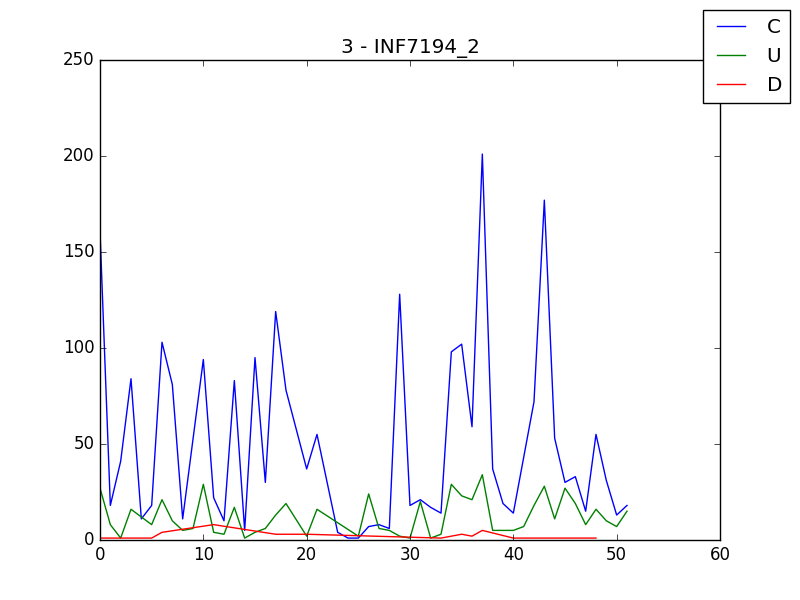
\includegraphics[width=\linewidth]{../src/exp_001_results/fig_3_INF7194_2_cud}
        \label{subfig:exp_001_3_cud}
    \end{subfigure}

    \caption
        [Exp 001 plots for C, U, and D activities]
        {Exp 001 plots for C, U, and D activities.}

    \label{fig:exp_001_cud}
\end{figure}
